% Please use the skeleton file you have received in the 
% invitation-to-submit email, where your data are already
% filled in. Otherwise please make sure you insert your 
% data according to the instructions in PoSauthmanual.pdf
\documentclass{PoS}

\title{Lensing studies using 21cm radiation from the EoR}

\ShortTitle{EoR 21cm lensing}

%\author{\speaker{First Author}\thanks{A footnote may follow.}\\
%        Author affiliation\\
%        E-mail: \email{author@email}}

\author{Robert Benton Metcalf\\
        Dipartimento di Fisica e Astronomia, Universit\'{a} di Bologna, viale B. Pichat 6/2 , 40127, Bologna, Italy\\
        E-mail: \email{robertbenton.metcalf@unibo.it}}

\author{Alkistis Pourtsidou\\
        Dipartimento di Fisica e Astronomia, Universit\'{a} di Bologna, viale B. Pichat 6/2 , 40127, Bologna, Italy\\
        E-mail: \email{alkistis.pourtsidou@unibo.it}}

\abstract{}

\FullConference{
Advancing Astrophysics with the Square Kilometre Array\\
June 8-13, 2014\\
Giardini Naxos, Italy}

\begin{document}

\section{Results}

It is possible that the EoR signal could be used to measure weak gravitational lensing.
In \cite{Zahn:2005ap} and \cite{Metcalf:2009}  it was shown that if the EoR is at redshift 
$z \sim 8$ or later, a large radio telescope such as the SKA could measure the lensing convergence power spectrum.  However a very large $f_{\rm sky}$ and a very compact low frequency array was assumed by those authors.  Here the calculation is repeated with parameters that are more consistent with current SKA plans.  The current plans for a 25 square degree survey with SKA\_Low will preclude measuring cosmological parameters through their effects on the weak lensing power-spectrum because of large sample variance.  (This is not true of the SKA\_Mid at lower redshift where the survey area will be much larger. See section *** for more details.)  It still might be possible to map the lensing convergence within the 25 square degree EoR survey area.  This would allow us to actually ``see'' the distribution of dark matter in a typical region of the sky, something that is only possible with galaxy lensing around very atypical, large galaxy clusters.  This would provide a great opportunity to correlate visible objects with mass and test the dark matter paradigm.

The previously mentioned authors extended the
Fourier-space quadratic estimator technique, which was first developed in 
\cite{Hu:2001tn} for CMB lensing  observations to three dimensional
observables, i.e. the $21$ cm intensity field $I(\theta,z)$.  
The  convergence
estimator and the corresponding lensing reconstruction noise are
calculated assuming that the temperature (brightness) distribution is
Gaussian. This will not be strictly true during the EoR, but serves as a reasonable approximation for these purposes. Note that the lensing reconstruction noise contains the thermal noise of the telescope which is calculated using the formula
\begin{equation}
C^{\rm N}_\ell = \frac{(2\pi)^3 T^2_{\rm sys}}{B t_{\rm obs} f^2_{\rm cover} \ell_{\rm max}(\nu)^2} \, ,
\end{equation} where the system temperature $T_{\rm sys}$ at high redshifts
 is dominated by galactic synchrotron radiation, $B$ is the chosen frequency window, $t_{\rm obs}$ the total observation time, $D_{\rm tel}$ the diameter (maximum baseline) of the core array, $\ell_{\rm max}(\lambda)=2\pi D_{\rm tel}/\lambda$ is the highest multipole that can be measured by the array at frequency $\nu$ (wavelength $\lambda$), and $f_{\rm cover}$ is the total collecting area of the core array $A_{\rm coll}$ divided by $\pi(D_{\rm tel}/2)^2$. 
 
 The advantage of 21cm lensing is that one is able to combine
information from multiple redshift slices. In Fourier space, the
temperature fluctuations are divided into perpendicular to the line of
sight wave vectors $\mathbf{k_\perp}=\mathbf{l}/r$, with $r$ the angular diameter distance to the source redshift, and a
discretized version of the parallel wave vector $k_\parallel =
\frac{2\pi}{{\cal L}}j$, where ${\cal L}$ is the depth of the observed
volume. Considering modes with different $j$ independent, an optimal
estimator can be found by combining the individual estimators for
different $j$ modes without mixing them. The three-dimensional lensing reconstruction noise is then found to be  \cite{Zahn:2005ap}\begin{equation}
N(L,\nu) =  \left[\sum_{j=1}^{j_{\rm max}} \frac{1}{L^4}\int \frac{d^2\ell}{(2\pi)^2}  \frac{[\mathbf{l} \cdot \mathbf{L} C_{\ell,j}+\mathbf{L} \cdot (\mathbf{L}-\mathbf{l})
C_{|\ell-L|,j}]^2}{2 C^{\rm tot}_{\ell,j}C^{\rm tot}_{|\mathbf{l}-\mathbf{L}|,j}}\right]^{-1}.
\end{equation}
Here, $C^{\rm tot}_{\ell,j}=C_{\ell,j}+C^{\rm N}_\ell$, where $C_{\ell,j}=[\bar{T}(z)]^2P_{\ell,j}$ with $\bar{T}(z)$ the mean observed brightness temperature at redshift $z$ due to the average HI density and $P_{\ell,j}$ the underlying dark matter power spectrum  \cite{Zahn:2005ap}. 
For SKA\_Low we can consider a $1,000~{\rm hr}$ observation time and we choose $B = 8 \, {\rm MHz}$ and $j_{\rm max}=40$, but with multiple bands $\nu$ that can be stacked to reduce the noise so that $N_L = 1/\displaystyle\sum_{\nu} [N(L,\nu)]^{-1}$. 
 
At redshift $z_s \sim 8$, we can assume the SKA1 Baseline Design \cite{Dewdney:2013} parameters of $A_{\rm coll} \simeq 0.3  \, {\rm km}^2$ with maximum baseline $D_{\rm tel}=4 \, {\rm km}$, while for SKA2 we can consider $A_{\rm coll} \simeq 1.2  \, {\rm km}^2$.
The estimated lensing noise is shown in Figure~\ref{fig:CLNL} along with the estimated signal.  
Here $C_L$ is the convergence field power spectrum at $z_s=8$ and $N_L$ the lensing reconstruction noise assuming a reionization fraction $f_{\rm HI}=1$.
\begin{figure}[h]
\centerline{
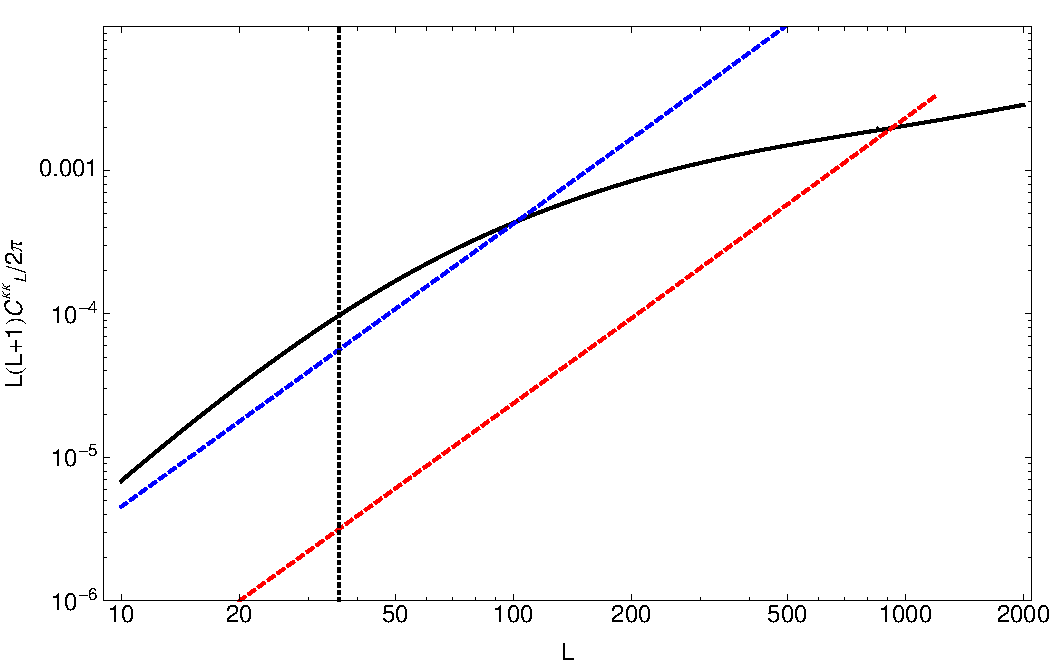
\includegraphics[scale=0.6]{tomographic_SKA_kappaPS.pdf}
}
\caption{The lensing convergence field power spectrum, $C_L$, for sources at $z=8$ is shown as a solid black line and lensing reconstruction noise $N_L$ as dashed lines.  The blue dashed curve is for the SKA1 Baseline Design with 10 8~MHz frequency bins around $z=8$ spanning the redshift range $z \simeq 6.5-11$.  The red line is for SKA2 and the same frequency bins. The vertical line is approximately the lowest $L$ accessible with a 5-by-5 degree field.  Where the noise curves are below $C_L$, typical fluctuations in the lensing deflection should be recoverable in a map. }
\label{fig:CLNL}
\end{figure}

These results show that it might be possible to map the lensing signal over a range of angular scales.  This measurement greatly benefits from the larger collecting area that will come with Phase 2 of the SKA (we also note that  considering a more compact array, i.e. smaller $D_{\rm tel}$, also improves the signal-to-noise).  The weak lensing power spectrum can be better measured for redshifts after reionization using SKA\_Mid and the same 21 cm intensity mapping technique discussed, but over a much larger area of sky \cite{PourtsidouMetcalf:2014}.\\

\begin{thebibliography}{99}

\bibitem{Zahn:2005ap}
 Zahn, O., \& Zaldarriaga, M., 2006, ApJ, 653, 922

\bibitem{Metcalf:2009}
Metcalf, R.~B., \& White, S.~D.~M., 2009, MNRAS, 394, 704

\bibitem{Hu:2001tn}
Hu, W., 2001, ApJ, 557, L79

\bibitem{Dewdney:2013}
Dewdney, P. (2013), SKA1 System Baseline Design, SKA Project Documents, (pp. 1-98)

\bibitem{PourtsidouMetcalf:2014}
Pourtsidou, A. \& {Metcalf}, R.~B., 2014, MNRAS, 439, L36-L40

\end{thebibliography}

\end{document}
